
\begin{frame}
    \begin{center}
        \center
        
\includegraphics[width=\textwidth]{figures/wrestlingNO3.png}
    \end{center}

    \Huge\bf
    \textcolor{msred}{
    Nitrate - the Classic}

\end{frame}


\begin{frame}
    \center 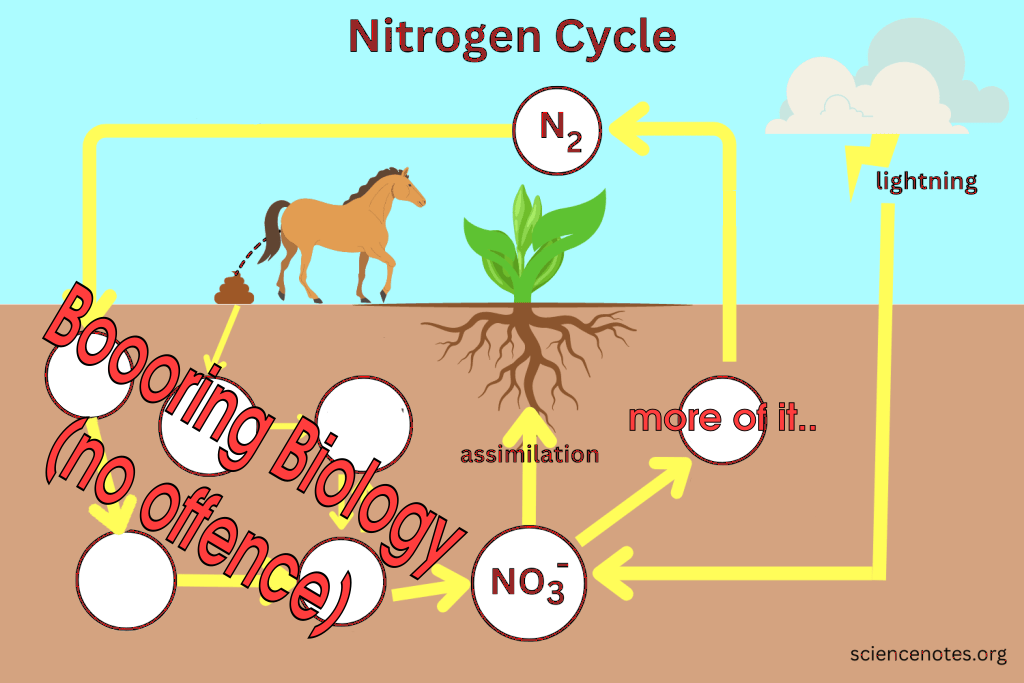
\includegraphics[width = \textwidth]{figures/Ncycle.png}
    \captionof*{figure}{Adapted from
    \tiny\url{https://sciencenotes.org/nitrogen-cycle/}}
\end{frame}

\begin{frame}
    \center 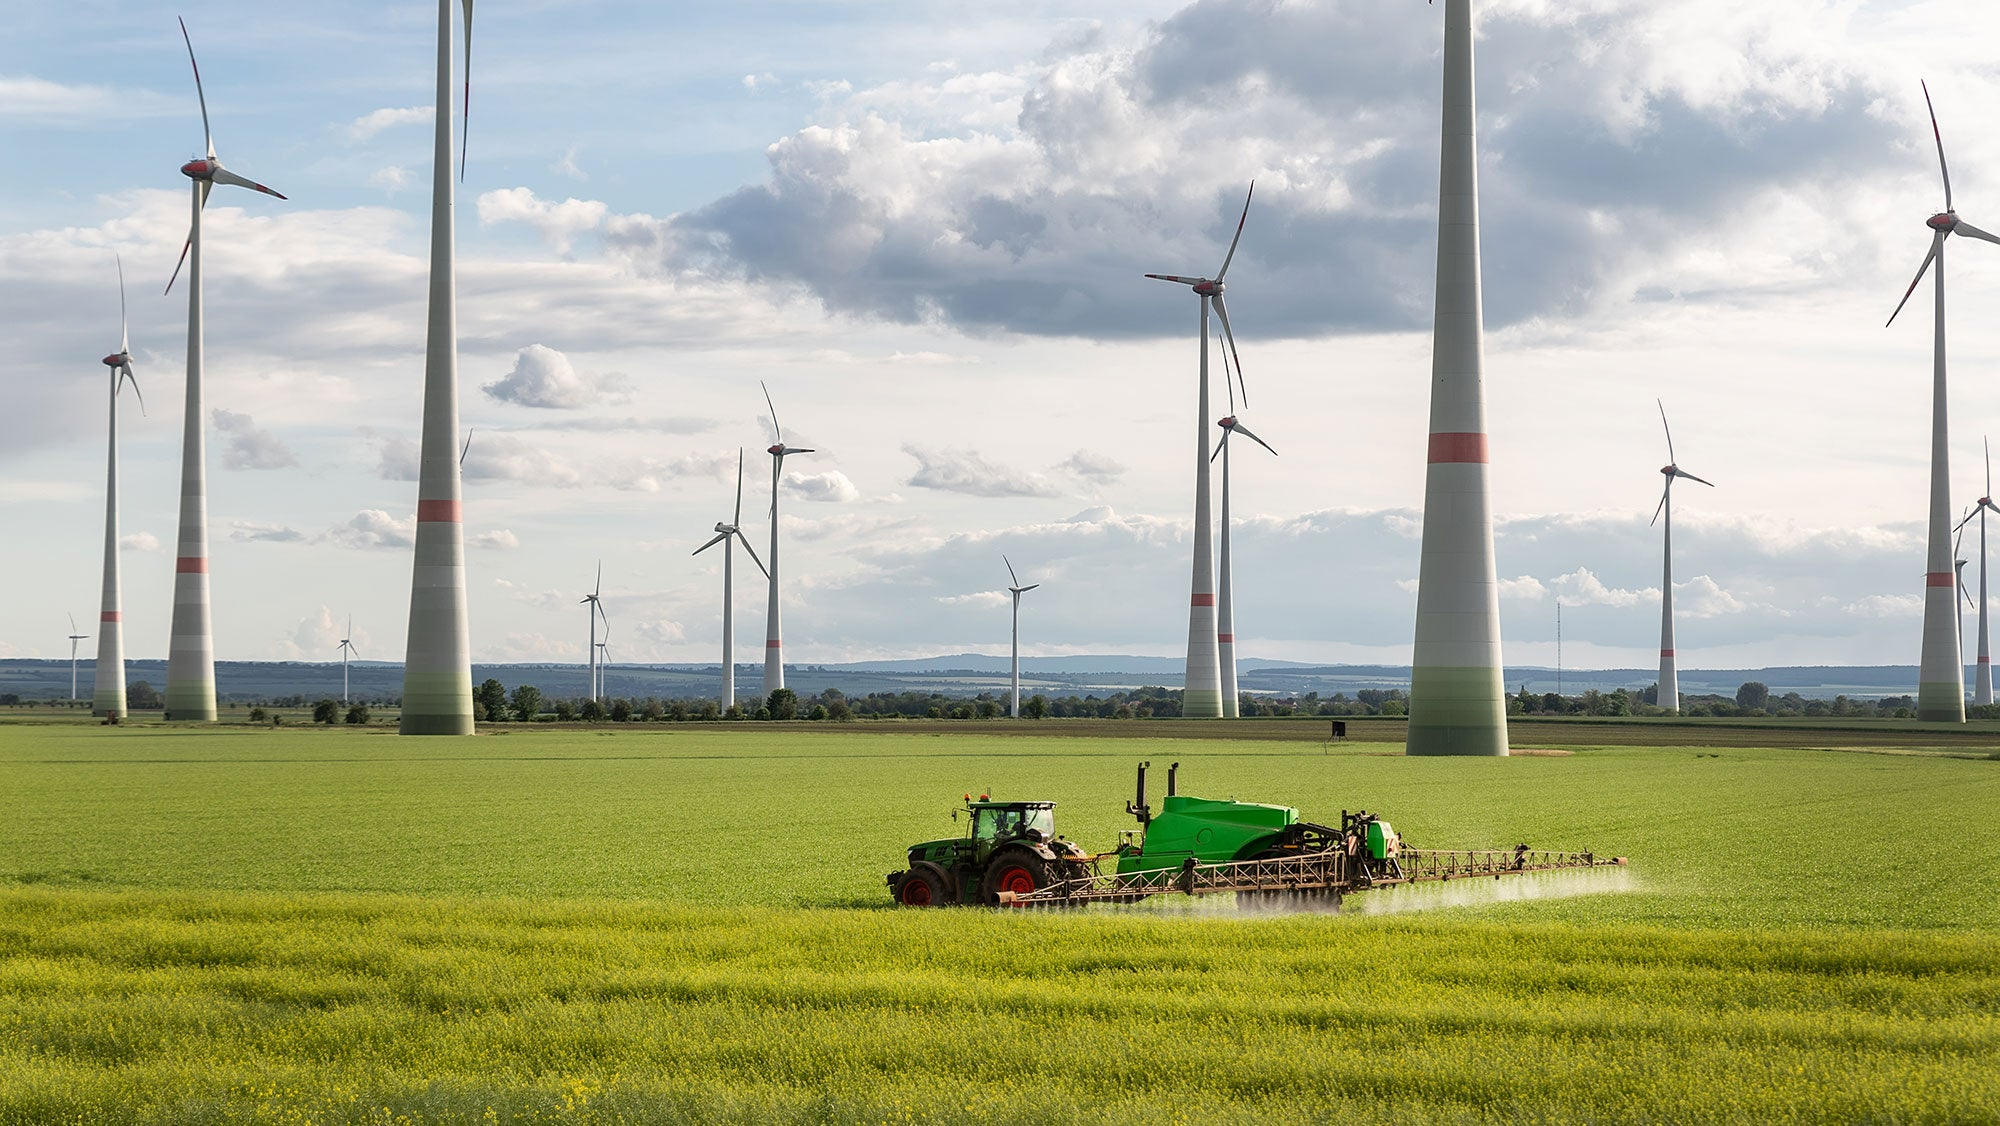
\includegraphics[width = .8\textwidth]{figures/farming.jpg}
\end{frame}

\begin{frame}
    \center 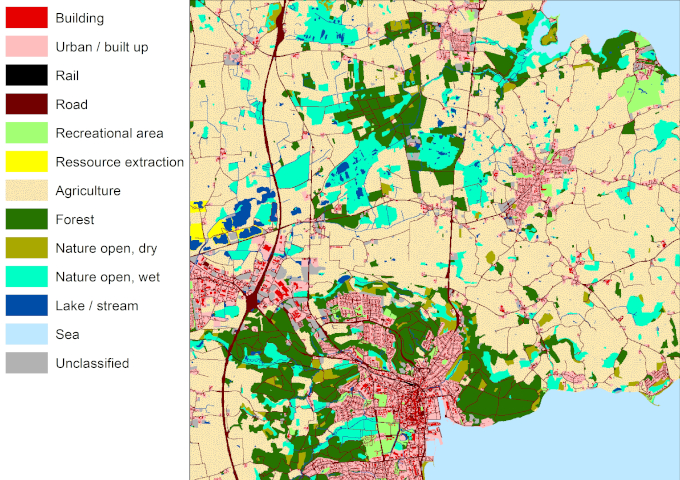
\includegraphics[width = .8\textwidth]{figures/farmland.jpg}

    More than half of the area of Denmark is used for
    agriculture!\footnote[frame]{\url{https://www.dst.dk/en/Statistik/emner/miljoe-og-energi/areal/arealopgoerelser}}
\end{frame}


\begin{frame}
\center\large
    Of that only 4 \% for direct human consumption\footnote[frame]{\url{https://www.dyrenesbeskyttelse.dk/artikler/danmark-har-verdens-stoerste-koedindustri}}!
\end{frame}


\begin{frame}{BREAKING: Farmers to be slightly less rich!}
    \begin{figure}
        \center
        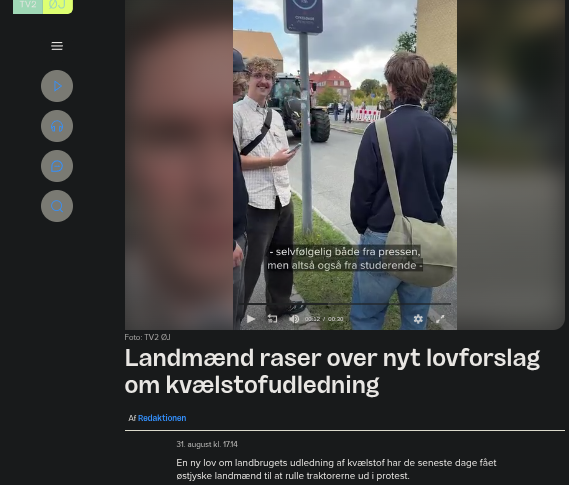
\includegraphics[width=\textwidth]{figures/tv2farmers}
    \end{figure}
\end{frame}

\begin{frame}{BREAKING: Farmers to be slightly less rich!}
    \begin{figure}
        \center
        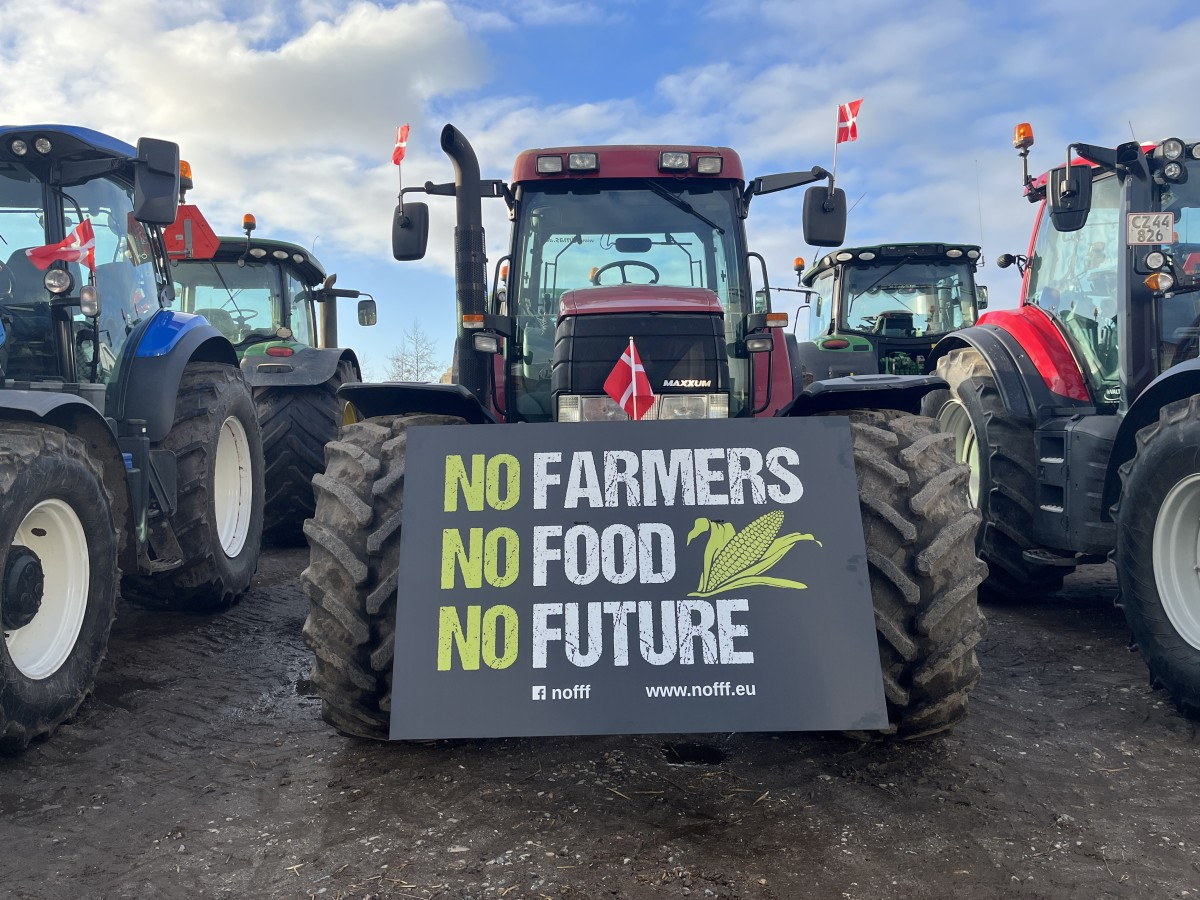
\includegraphics[width=\textwidth]{figures/nofnofnof.jpeg}
    \end{figure}
\end{frame}

\begin{frame}{BREAKING: Farmers to be slightly less rich!}
    \textbf{Food waste in Denmark}
    \begin{description}
        \item[Sumtotal]  881.062 tons / year
            \begin{description}
                \item[Food industry] 457,172 metric tons /
                    year (51,9\%)
                \item[Households] 235,000 metric tons / year (26,7\%)
                \item[Detail og engros] 103,906 metric tons / year (11,8\%)
                \item[Primary production]  42,984 metric tons / year (4,9 \%)
                \item[Service sector] 42,000 metric tons / year (4,8 \%)
            \end{description}
    \end{description}

    \footnotesize
    \url{https://stopspildafmad.org/om-madspild/madspild-i-tal/}

\end{frame}

\begin{frame}{Meet the meat that really should meet its end}
    \begin{figure}
        \center
        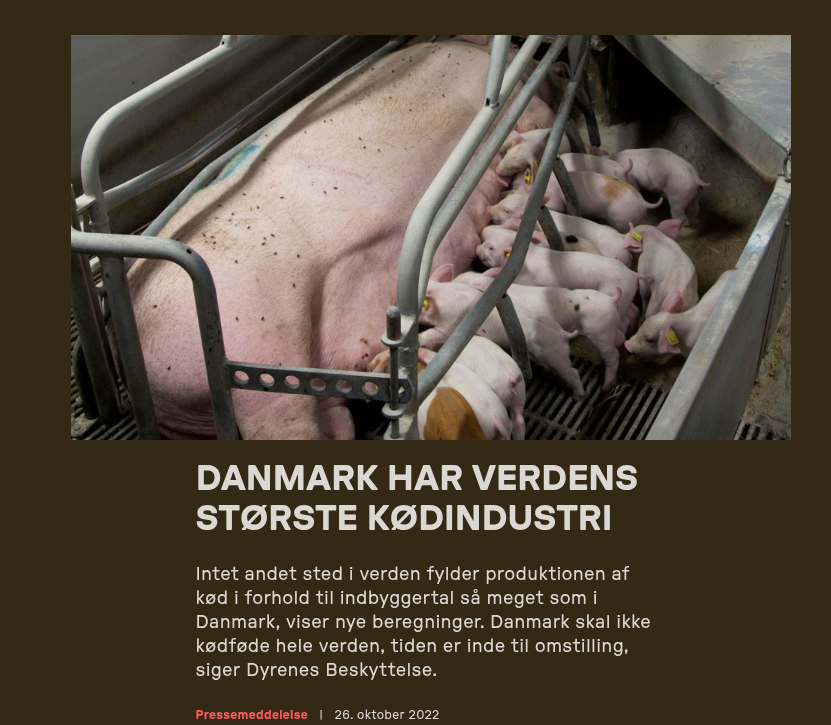
\includegraphics[width=.5\textwidth]{figures/dyrensebeskyttelse_koedprod.jpg}
    \end{figure}
    \footnotesize
    \url{https://www.dyrenesbeskyttelse.dk/artikler/danmark-har-verdens-stoerste-koedindustri}
\end{frame}

\begin{frame}{Meet the meat that really should meet its end}
    \begin{multicols}{2}
        \begin{minipage}{.5\textwidth}
        \center
        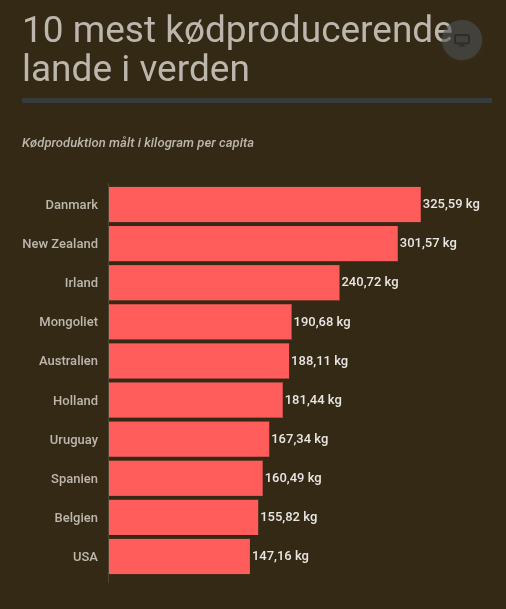
\includegraphics[width=.75\textwidth]{figures/meatprod.jpg}
    \end{minipage}\columnbreak
        \vspace{4em}
or \textcolor{msred}{$\sim 1.92$ mio metric tons / year}. 
        Exports \textcolor{msred}{$\sim85\%$} to \textcolor{msred}{$90\%$}\footnote[frame]{
        \url{https://www.dyrenesbeskyttelse.dk/artikler/danmark-har-verdens-stoerste-koedindustri}}
    \end{multicols}
\end{frame}

\begin{frame}{BREAKING: Farmers to be slightly less rich!}
    \begin{figure}
        \center
        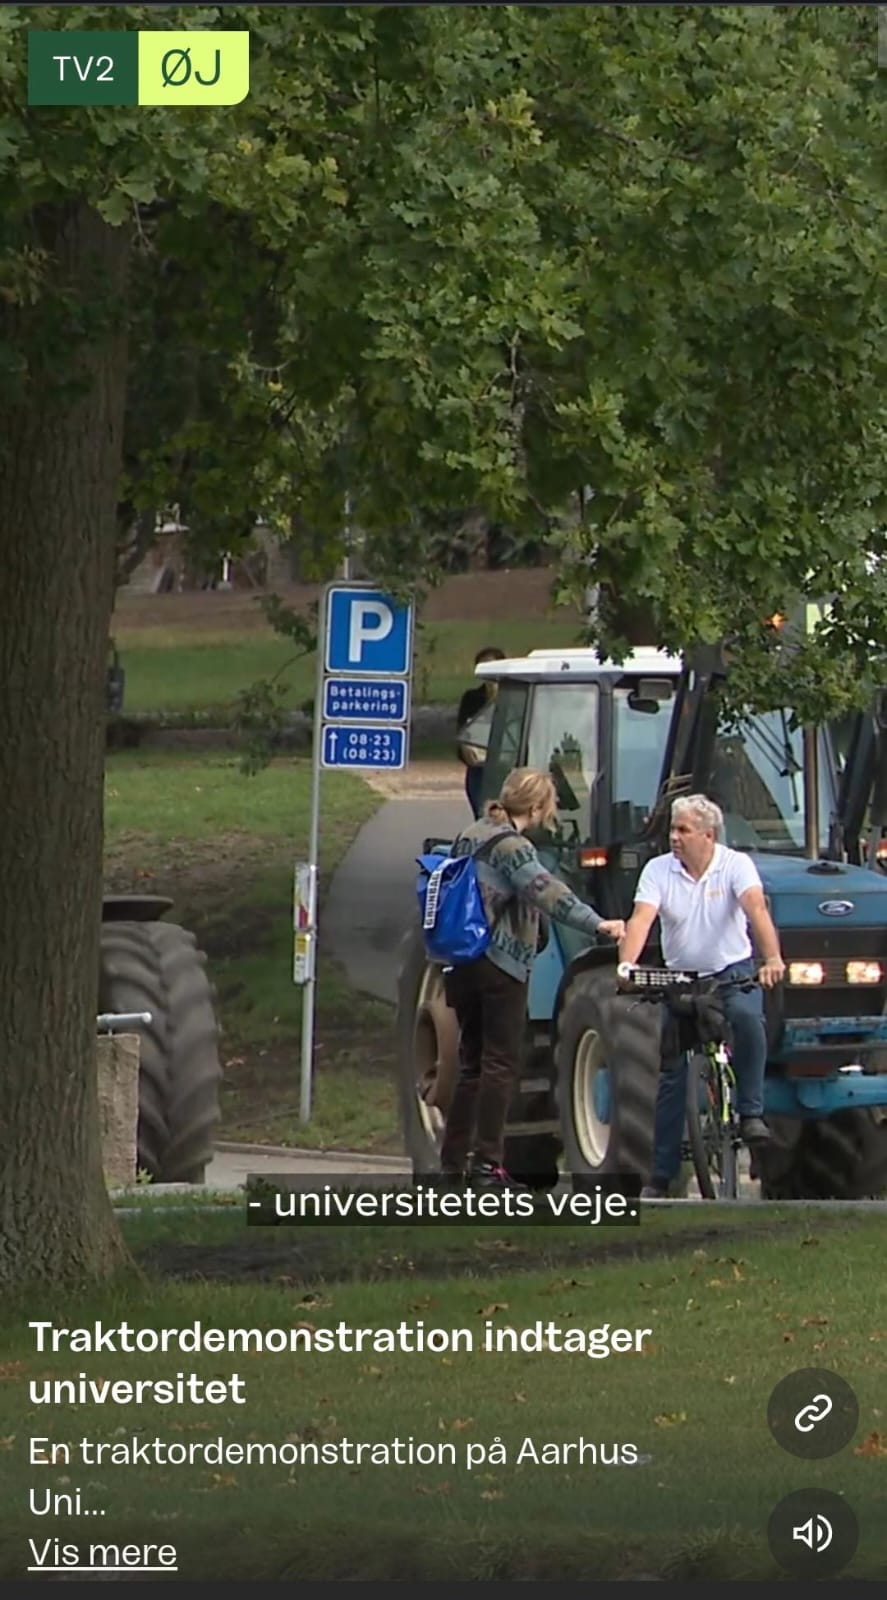
\includegraphics[width=.5\textwidth]{figures/me}
    \end{figure}
\end{frame}



\begin{frame}{Consequences}
    \begin{description}
        \item[Environmental]
            Pollution of bodies of water. Excess algae
            growth, extinction of fauna, etc.



        \item<2->[Health]
            Nitrate in drinking water has been linked to
            methemoglobinemia (blue-baby-syndrome),
            colorectal cancer, thyroid disease, and
            more~\cite{ward_drinking_2018, jacobsen_health-economic_2024}.

            Increased risk even below regulatory
            limits~\cite{ward_drinking_2018}!
    \end{description}
\end{frame}

\begin{frame}{Consequences from the tab}


    \emph{
        For over 60 years, the global guideline for nitrates in drinking water
        has been 50 milligrams per litre (mg/L) [...] set in
        the 1950s\footnote[frame]{\tiny
    \url{https://www.greenpeace.org/international/story/82511/industrial-agriculture-profits-toxic-nitrates-pollution-tap-water/}}.}

    \end{frame}

\begin{frame}
    \textcolor{msred}{\large This limit is hopelessly out of date}\vspace{1em}

    Literature proposes lower limits of $<10\%$, reducing the risk by $15\%$.
    Even lower limits of $<4\%$ bring this number down
    further~\cite{jacobsen_health-economic_2024, schullehner_nitrate_2018}.

\end{frame}

\begin{frame}{Blue babies (not good)}
    \begin{multicols}{2}
        \begin{minipage}{\columnwidth}
            {
                \centering
                
\includegraphics[width=.9\textwidth]{figures/rekt}
            }
        \end{minipage}
        \columnbreak

        \textbf{Infant methemoglobinemia}
        \begin{itemize}
            \item Can progress to cause coma and death if not left
                untreated~\cite{knobeloch_blue_2000,
                chen_methemoglobinemia_2026}.

            \item 2 cases where water for formula contained
                concentrations of \textcolor{msred}{\bf roughly half}
                of the 'save limit~\cite{knobeloch_blue_2000}'.

        \end{itemize}
    \end{multicols}
\end{frame}

\begin{frame}{Nitrate pollution in Denmark}
    \center 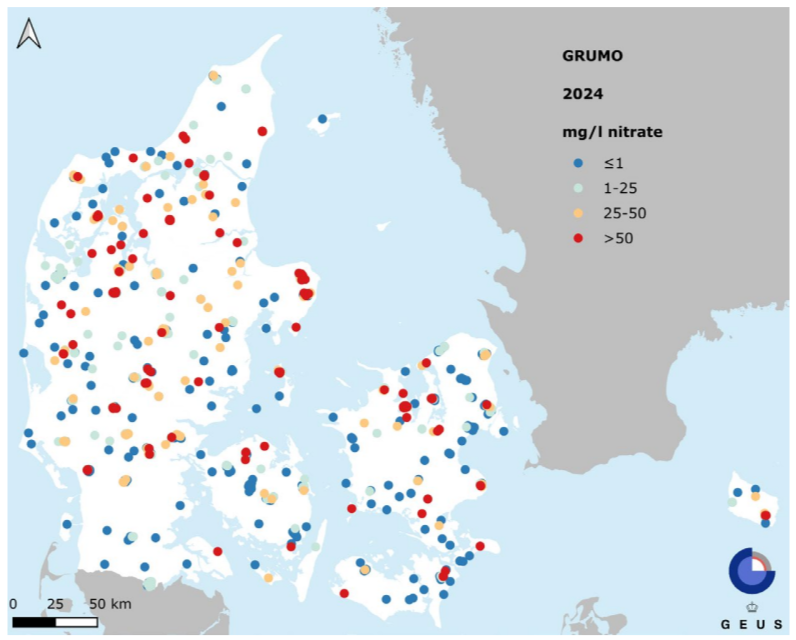
\includegraphics[width = .8\textwidth]{figures/grumoMapNitrate.png}
    \captionof{figure}{ \footnotesize From GEUS' groundwater report
    2025~\cite{laerke_thorling_groundwater_2025}.}
\end{frame}

\begin{frame}{Mixing and exploting}
    \center 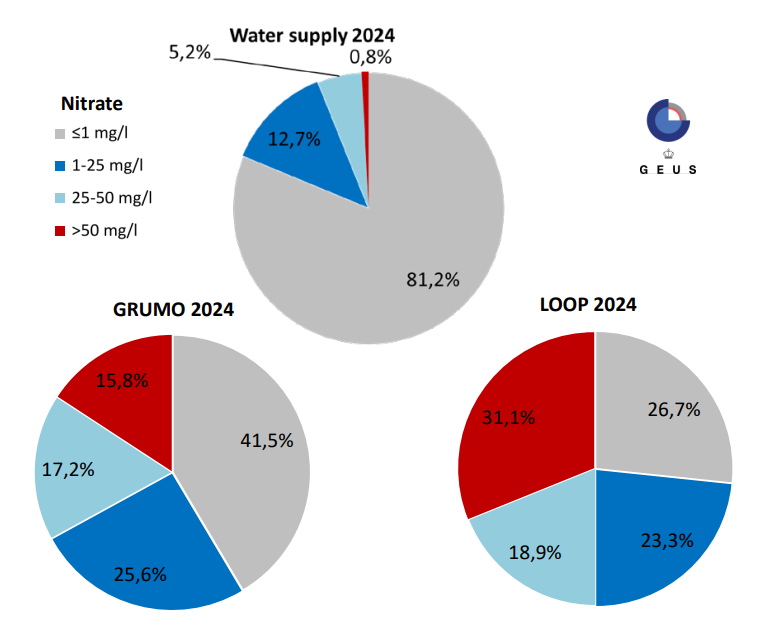
\includegraphics[width = .8\textwidth]{figures/nitrateCakes.png}
    \captionof{figure}{ \footnotesize From GEUS' groundwater report
    2025~\cite{laerke_thorling_groundwater_2025}.}
\end{frame}

